\documentclass{article}
\usepackage{fullpage}
\usepackage[english,greek, main=greek]{babel}
\usepackage[utf8]{inputenc}

\usepackage{amsmath}
\usepackage{bm}
\usepackage{chngcntr}
\counterwithin{equation}{section}

\usepackage{graphicx}
\usepackage{subcaption}
\usepackage{placeins}

\usepackage{verbatim}
\usepackage{booktabs}

\newcommand{\eng}[1]{\foreignlanguage{english}{#1}}
\newcommand{\Alpha}{\mathrm{A}}

\useshorthands{;}
\defineshorthand{;}{?}

\title{Όραση Υπολογιστών\\
\large Εργαστήριο 1}
\author{Αναστάσιος Στέφανος Αναγνώστου\\
    \texttt{03119051}
    \and
    Σπυρίδων Παπαδόπουλος\\
\texttt{03119058}}

\date{7 Απριλίου 2023}

\begin{document}
\maketitle

\clearpage
\tableofcontents
\clearpage

Ο κώδικας παρατίθεται σε ξεχωριστά αρχεία με επαρκή σχολιασμό και όχι στην παρούσα αναφορά.

\section{Μέρος 1}

Στο πρώτο μέρος του εργαστηρίου υλοποιείται σύστημα παρακολούθησης προσώπου και χεριών σε βίντεο νοηματικής γλώσσας.

\subsection{Ανίχνευση Δέρματος Προσώπου και Χεριών}

Η ανίχνευση δέρματος προσώπου και χεριών επιτυγχάνεται χρήσει ενός πιθανοτικού ανιχνευτή ανθρωπίνου δέρματος. Συγκεκριμένα, θεωρείται ότι το χρώμα του δέρματος μοντελοποιείται με μία διδιάστατη Γκαουσιανή κατανομή.

\begin{equation}
    P(\pmb{c} = skin) = \frac{1}{\sqrt{\left| \Sigma \right| (2\pi)^2}}e^{-\frac{1}{2}(\pmb{c}-\pmb{\mu}) \Sigma^{-1}(\pmb{c}-\pmb{\mu})^{T}}
\end{equation}

Το διάνυσμα τιμών $\vec{c}$ της κατανομής είναι οι διαστάσεις $C_b, C_r$ του χρωματικού χώρου \eng{YCbCr}, δηλαδή:

\begin{equation}
    \pmb{c} = \begin{bmatrix} C_b & C_r \end{bmatrix}^{T} 
\end{equation}

Η συνάρτηση πυκνότητας πιθανότητας εκπαιδεύεται χρήσει των παρεχόμενων δεδομένων \texttt{\eng{skinSamplesRGB.mat}}. Φυσικά, προτού χρησιμοποιηθούν, πρέπει να μετασχηματιστούν από τον χώρο \eng{RGB} στον χώρο \eng{YCbCr}. Αφού εκπαιδευτεί η συνάρτηση πυκνότητας πιθανότητας, η δυαδική εικόνα ανίχνευσης δέρματος προκύπτει, με κατάλληλη κατωφλιοποίηση, ως:

\begin{equation}
    \begin{gathered}
        I(x, y) =
        \begin{cases}
            1, \underset{x, y}{\arg} \left\{P(\pmb{c}(x, y) = skin)\ge \theta\right\} \\
            0, \text{ειδάλλως}
        \end{cases}
    \end{gathered}
\end{equation}

Σε αυτό το σημείο, η δυαδική εικόνα έχει μερικά κενά, τα οποία είναι ανεπιθύμητα, αφού είναι γνωστό ότι οι περιοχές δέρματος είναι συνεχείς. Αυτό επαληθεύεται από την ακόλουθη εικόνα \ref{fig:binary-skin-bad}.

\begin{figure*}[h]
    \centering
    \begin{subfigure}[b]{0.49\textwidth}
        \centering
        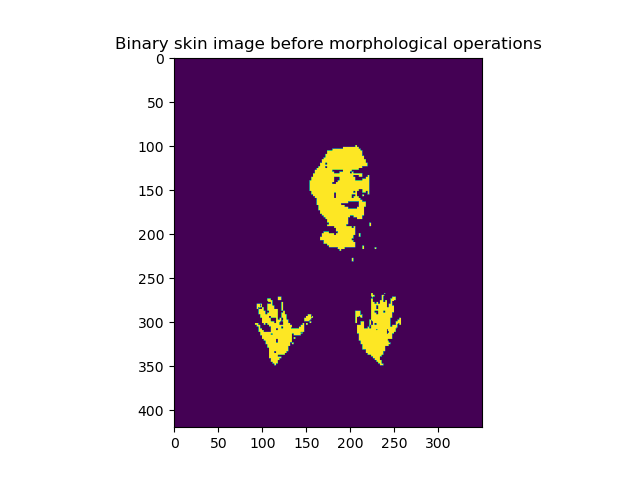
\includegraphics[width=\textwidth]{../part1/results/binary_skin_image.png}
        \caption{Η ατελής δυαδική εικόνα δέρματος}
        \label{fig:binary-skin-bad}
    \end{subfigure}
    \hfill
    \begin{subfigure}[b]{0.49\textwidth}
        \centering
        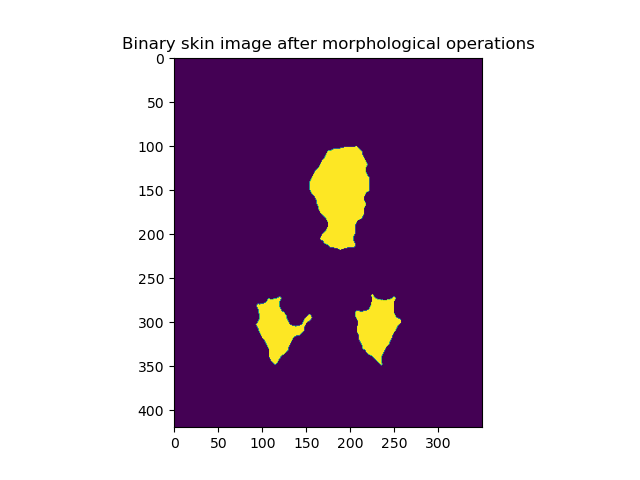
\includegraphics[width=\textwidth]{../part1/results/binary_skin_image_better.png}
        \caption{Η βελτιωμένη δυαδική εικόνα δέρματος}
        \label{fig:binary-skin-good}
    \end{subfigure}
\end{figure*}


Για την εξάλειψη των κενών, εφαρμόζεται \eng{opening} με ένα πολύ μικρό δομικό στοιχείο και \eng{closing} με ένα μεγαλύτερο ($\times 6$) δομικό στοιχείο. Το αποτέλεσμα παρατίθεται στην εικόνα \ref{fig:binary-skin-good}.

Παρατηρείται ότι οι περιοχές είναι τώρα συνεχείς και η απεικόνιση σαφώς βελτιωμένη, με τίμημα την ακρίβεια σε οριακές περιοχές όπως είναι τα δάχτυλα. 

Τέλος, θα δημιουργηθούν ορθογώνια τα οποία περιβάλλουν τις περιοχές ενδιαφέροντος. Παρουσιάζονται ενδεικτικά μερικά πλαίσια από το βίντεο στην εικόνα \ref{fig:skin-detection}.

\begin{figure*}
    \centering
    \begin{subfigure}[b]{0.49\textwidth}
        \centering
        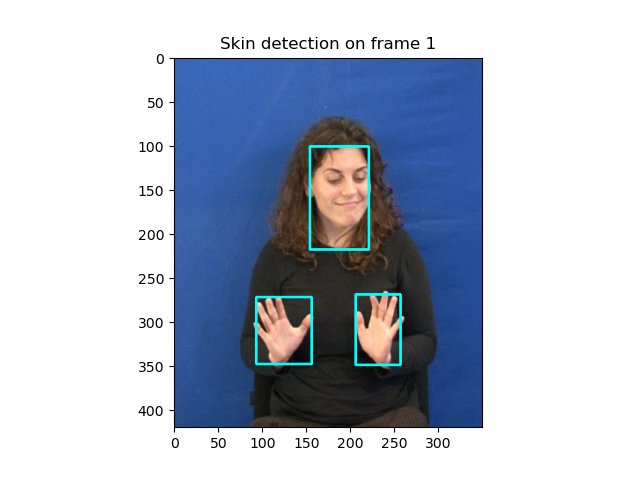
\includegraphics[width=\textwidth]{../part1/results/skin_detection_1.png}
        \caption{Πλαίσιο 1}
        \label{fig:}
    \end{subfigure}
    \hfill
    \begin{subfigure}[b]{0.49\textwidth}  
        \centering 
        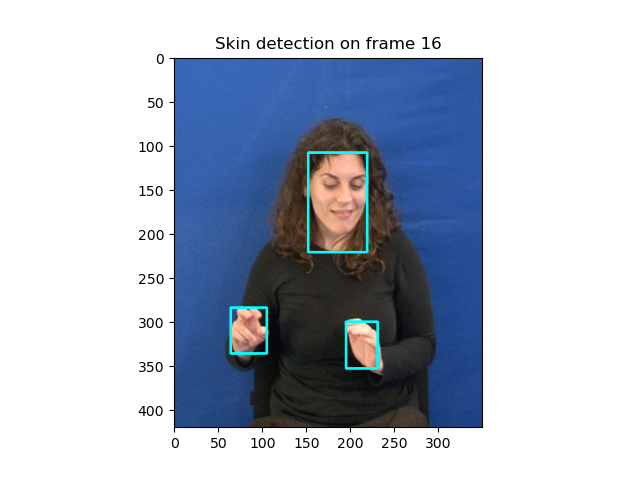
\includegraphics[width=\textwidth]{../part1/results/skin_detection_16.png}
        \caption{Πλαίσιο 16}
        \label{fig:}
    \end{subfigure}
    \vskip\baselineskip
    \begin{subfigure}[b]{0.49\textwidth}   
        \centering 
        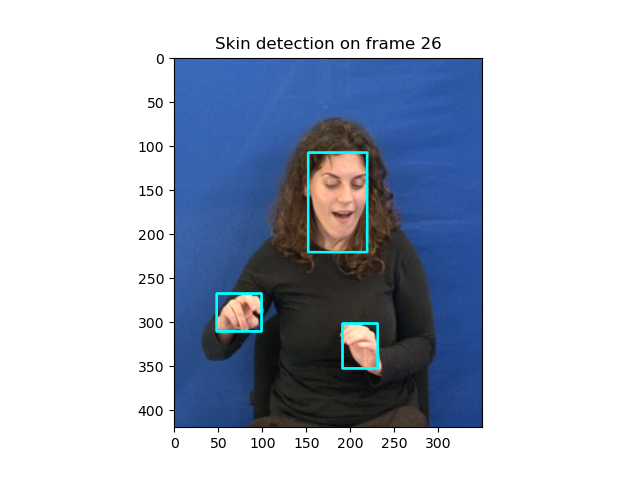
\includegraphics[width=\textwidth]{../part1/results/skin_detection_26.png}
        \caption{Πλαίσιο 26}
        \label{fig:}
    \end{subfigure}
    \hfill
    \begin{subfigure}[b]{0.49\textwidth}   
        \centering 
        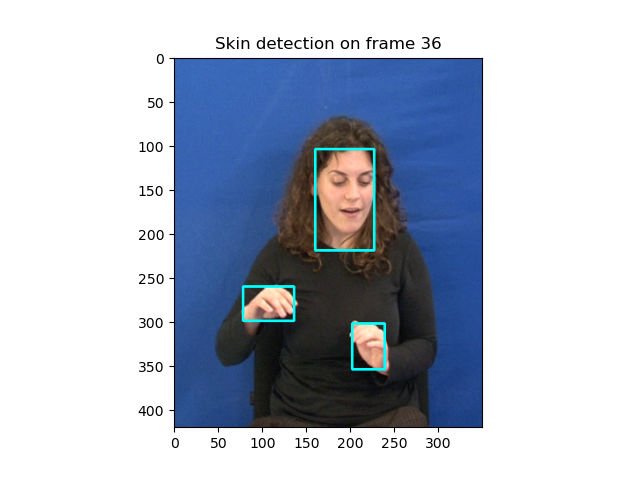
\includegraphics[width=\textwidth]{../part1/results/skin_detection_36.png}
        \caption{Πλαίσιο 36}
        \label{fig:}
    \end{subfigure}
    \caption{Ενδεικτικός εντοπισμός δέρματος σε μερικά πλαίσια}
    \label{fig:skin-detection}
\end{figure*}
\FloatBarrier

Φαίνεται, ότι τα αποτελέσματα είναι αρκετά ικανοποιητικά. Συγκεκριμένα, οι περιοχές εντοπίζονται με αρκετή ακρίβεια σε όλες τις περιπτώσεις και τα χέρια παρακολουθούνται επιτυχώς, παρότι κινούνται και αλλάζουν το σχήματος. Μάλιστα, όπως αλλάζει το φαινόμενο μέγεθος των χεριών, αλλάζει μαζί και το περιβάλλον κουτί.


\clearpage
\subsection{Παρακολούθηδη Προσώπου και Χεριών}

Σε αυτό το σημείο θα επιχειρηθεί η παρακολούθηση του προσώπου και των χεριών, όχι όμως μέσω ανίχνευσης δέρματος, αλλά μέσω εκτίμησης οπτικής ροής. Αντί, δηλαδή, να βρίσκεται σε καθένα πλαίσιο εκ νέου η περιοχή γύρω από το δέρμα, γίνεται μία εκτίμηση της οπτικής ροής από πλαίσιο σε πλαίσιο.

\subsubsection{Υλοποίηση Αλγορίθμου \eng{Lucas-Kanade}}

Η εκτίμηση της οπτικής ροής, εν προκειμένω, θα γίνει χρήσει του αλγορίθμου \eng{Lucas-Kanade}. Κατά τον αλγόριθμο αυτόν, υπολογίζεται η οπτική ροή καθενός σημείου της εικόνας, χρήσει της μεθόδου ελαχίστων τετραγώνων, υπό την παραδοχή ότι αυτή παραμένει σταθερή σε μία μικρή περιοχή γύρω από το σημείο.

\begin{equation}
    \begin{gathered}
        I_n(\pmb{x}) \approx I_{n-1}(\pmb{x+d})\overset{\text{\eng{Taylor}}}{\Rightarrow} \\ 
        I_{n-1}(\pmb{x+d}) \approx I_{n-1}(\pmb{x+d_i}) + \nabla I_{n-1}(\pmb{x+d_i})^{T}\pmb{u}
    \end{gathered}
\end{equation}

Ελαχιστοποιώντας το τετραγωνικό σφάλμα, προκύπτει ένα σύστημα το οποίο προσδιορίζει πλήρως την βελτίωση της εκτίμησης της οπτικής ροής.

Ο αλγόριθμος δεν εφαρμόζεται σε κάθε σημείο της εικόνας, αλλά αποδεικνύεται (απλώς κοιτάζοντας το προκύπτον σύστημα) ότι δίνει την βέλτιστη εκτίμηση όταν εφαρμόζεται σε γωνίες. Επομένως, πρώτα γίνεται εντοπισμός γωνιών στην εικόνα και έπειτα εφαρμόζεται ο αλγόριθμος. Η εφαρμογή γίνεται επαναληπτικά ανά σημείο, μέχρις ότου, είτε δύο διαδοχικές βελτιώσεις να διαφέρουν κατά αμελητέο ποσό, είτε να ξεπεραστεί κάποιο όριο επαναλήψεων.

Παρατίθενται ενδεικτικά πλαίσια για την αξιολόγηση της μεθόδου στην εικόνα \ref{fig:tracking1}. Σημειώνεται, επίσης, ότι στα αρχεία της αναφοράς δίνεται το αποτέλεσμα της συνένωσης όλων των πλαισίων σε μορφή \texttt{\eng{gif}}.

\begin{figure*}[h]
    \centering
    \begin{subfigure}[b]{0.49\textwidth}
        \centering{}
        \includegraphics[width=\textwidth]{../part1/flow/n_16.png}
        \caption{Πλαίσιο 16}
        \label{fig:}
    \end{subfigure}
    \hfill
    \begin{subfigure}[b]{0.49\textwidth}  
        \centering 
        \includegraphics[width=\textwidth]{../part1/flow/n_26.png}
        \caption{Πλαίσιο 26}
        \label{fig:}
    \end{subfigure}
    \caption{Ενδεικτικός εντοπισμός δέρματος χρήσει εκτίμησης οπτικής ροής}
    \label{fig:tracking1}
\end{figure*}
\begin{figure*}[h]
    \begin{subfigure}[b]{0.49\textwidth}   
        \centering 
        \includegraphics[width=\textwidth]{../part1/flow/n_36.png}
        \caption{Πλαίσιο 36}
        \label{fig:}
    \end{subfigure}
    \hfill
    \begin{subfigure}[b]{0.49\textwidth}   
        \centering 
        \includegraphics[width=\textwidth]{../part1/flow/n_46.png}
        \caption{Πλαίσιο 46}
        \label{fig:}
    \end{subfigure}
    \caption{Ενδεικτικός εντοπισμός δέρματος χρήσει εκτίμησης οπτικής ροής}
    \label{fig:tracking2}
\end{figure*}
\FloatBarrier

Επισκοπώντας τα αποτελέσματα, συμπεραίνεται, ότι η εκτίμηση της οπτικής ροής λειτουργεί αρκετά καλά για μικρές, αργές κινήσεις. Αυτό επαληθεύεται από τα 3 πρώτα παρατιθέμενα πλαίσια, στα οποία οι κινήσεις ήταν αργές και ομαλές. Ωστόσο, όταν οι κινήσεις γίνονται απότομες, η αποδοτικότητα του αλγορίθμου μειώνεται, με αποτέλεσμα να υστερούν τα κουτιά από τις περιοχές ενδιαφέροντος, όπως φαίνεται στο τελευταίο πλαίσιο. Σημειώνεται, επίσης, ότι η κλίμακα του κουτιού δεν αλλάζει, όπως προηγουμένως, αλλά παραμένει σταθερή.

\clearpage
\subsubsection{Υπολογισμός Μετατόπισης Παραθύρων και Οπτικής Ροής}

Το συνολικό διάνυσμα μετατόπισης του κουτιού βρίσκεται, ουσιαστικά, υπολογίζοντας έναν απλό μέσον όρο. Συγκεκριμένα, υπολογίζεται ο μέσος όρος των διανυσμάτων μετατόπισης αυτών, τα οποία έχουν ενέργεια $\left|\left| \pmb{d}^2 \right|\right| = d_x^2 + dy^2$ μεγαλύτερη από ένα κατώφλι, ώστε να απορριφθούν \eng{outliers} και να επιτευχθεί καλύτερη ακρίβεια.

\begin{figure*}[h]
    \centering
    \begin{subfigure}[b]{0.49\textwidth}
        \centering{}
        \includegraphics[width=\textwidth]{../part1/flow/16.png}
        \caption{Πλαίσιο 16}
        \label{fig:}
    \end{subfigure}
    \hfill
    \begin{subfigure}[b]{0.49\textwidth}  
        \centering 
        \includegraphics[width=\textwidth]{../part1/flow/26.png}
        \caption{Πλαίσιο 26}
        \label{fig:}
    \end{subfigure}
    \caption{Εντοπισμός δέρματος και οπτική ροή σε μερικά πλαίσια}
    \label{fig:flows1}
\end{figure*}
\begin{figure*}[h]
    \begin{subfigure}[b]{0.49\textwidth}   
        \centering 
        \includegraphics[width=\textwidth]{../part1/flow/36.png}
        \caption{Πλαίσιο 36}
        \label{fig:}
    \end{subfigure}
    \hfill
    \begin{subfigure}[b]{0.49\textwidth}   
        \centering 
        \includegraphics[width=\textwidth]{../part1/flow/46.png}
        \caption{Πλαίσιο 46}
        \label{fig:}
    \end{subfigure}
    \caption{Εντοπισμός δέρματος και οπτική ροή σε μερικά πλαίσια}
    \label{fig:flows2}
\end{figure*}


\clearpage
\subsubsection{Πολυ-κλιμακωτός Υπολογισμός Οπτικής Ροής}

Η κακή επίδοση του αλγορίθμου στις απότομες δημιουργεί την ανάγκη επέκτασής του σε περισσότερες κλίμακες. Συγκεκριμένα, η πολυκλιμακωτή εκδοχή του, αναλύει την αρχική εικόνα σε μία Γκαουσιανή πυραμίδα εικόνων, στο καθένα επίπεδο της οποίας βρίσκεται μία υποδειγματοληπτημένη εκδοχή της αυθεντικής εικόνας. Σε καθεμία κλίμακα χρησιμοποιείται ο αυθεντικός αλγόριθμος και μεταφέρει την εκτίμησή του στην αμέσως ανώτερη κλίμακα, προσαρμόζοντάς την κατάλληλα. Σημειώνεται, ότι τα χαρακτηριστικά πρέπει τώρα να εξαχθούν για κάθε επίπεδο της κλίμακας, όχι μόνο για την αρχική εικόνα. 

\begin{figure*}[h]
    \centering
    \begin{subfigure}[b]{0.49\textwidth}
        \centering{}
        \includegraphics[width=\textwidth]{../part1/flow_multiscale/n_16.png}
        \caption{Πλαίσιο 16}
        \label{fig:}
    \end{subfigure}
    \hfill
    \begin{subfigure}[b]{0.49\textwidth}  
        \centering 
        \includegraphics[width=\textwidth]{../part1/flow_multiscale/n_26.png}
        \caption{Πλαίσιο 26}
        \label{fig:}
    \end{subfigure}
    \caption{Ενδεικτικός πολυκλιμακωτός εντοπισμός δέρματος χρήσει εκτίμησης οπτικής ροής}
    \label{fig:tracking_multiscale1}
\end{figure*}
\begin{figure*}[h]
    \begin{subfigure}[b]{0.49\textwidth}   
        \centering 
        \includegraphics[width=\textwidth]{../part1/flow_multiscale/n_36.png}
        \caption{Πλαίσιο 36}
        \label{fig:}
    \end{subfigure}
    \hfill
    \begin{subfigure}[b]{0.49\textwidth}   
        \centering 
        \includegraphics[width=\textwidth]{../part1/flow_multiscale/n_46.png}
        \caption{Πλαίσιο 46}
        \label{fig:}
    \end{subfigure}
    \caption{Ενδεικτικός πολυκλιμακωτός εντοπισμός δέρματος χρήσει εκτίμησης οπτικής ροής}
    \label{fig:tracking_multiscale2}
\end{figure*}
\FloatBarrier

Παρατηρείται, ότι σε κάθε πλαίσιο ο εντοπισμός είναι ακριβέστερος. Η διαφορά είναι ιδιαίτερα αξιοσημειώτη στο τελευταίο παρατιθέμενο πλαίσιο, όπου το μπλε κουτί περικυκλώνει τέλεια το αριστερό χέρι, ενώ στην μονοκλιμακωτή εκδοχή το έχανε λόγω ταχύτητας.

Παρακάτω δίνονται τα αντίστοιχα αποτελέσματα για την απεικόνιση της οπτικής ροής. Η βελτίωση της ποιότητας είναι ορατή και εκεί, αφού τα διανύσματα οπτικής ροής είναι πλέον πολύ ομοιόμορφα και όλα σαφώς προσανατολισμένα προς κάποια κατεύθυνση, σε αντίθεση με την προηγούμενη μέθοδο όπου υπήρχαν κάποιες διακυμάνσεις. 

\begin{figure*}[h]
    \centering
    \begin{subfigure}[b]{0.49\textwidth}
        \centering{}
        \includegraphics[width=\textwidth]{../part1/flow_multiscale/16.png}
        \caption{Πλαίσιο 16}
        \label{fig:}
    \end{subfigure}
    \hfill
    \begin{subfigure}[b]{0.49\textwidth}  
        \centering 
        \includegraphics[width=\textwidth]{../part1/flow_multiscale/26.png}
        \caption{Πλαίσιο 26}
        \label{fig:}
    \end{subfigure}
    \caption{Πολυκλιμακωτός εντοπισμός δέρματος και οπτική ροή σε μερικά πλαίσια}
    \label{fig:flow_multiscales1}
\end{figure*}
\begin{figure*}[h]
    \begin{subfigure}[b]{0.49\textwidth}   
        \centering 
        \includegraphics[width=\textwidth]{../part1/flow_multiscale/36.png}
        \caption{Πλαίσιο 36}
        \label{fig:}
    \end{subfigure}
    \hfill
    \begin{subfigure}[b]{0.49\textwidth}   
        \centering 
        \includegraphics[width=\textwidth]{../part1/flow_multiscale/46.png}
        \caption{Πλαίσιο 46}
        \label{fig:}
    \end{subfigure}
    \caption{Πολυκλιμακωτός εντοπισμός δέρματος και οπτική ροή σε μερικά πλαίσια}
    \label{fig:flow_multiscales2}
\end{figure*}

\clearpage
\section{Μέρος 2}


\clearpage
\section{Μέρος 3}


\end{document}
